% Generated by Sphinx.
\def\sphinxdocclass{report}
\documentclass[letterpaper,10pt,english]{sphinxmanual}
\usepackage[utf8]{inputenc}
\DeclareUnicodeCharacter{00A0}{\nobreakspace}
\usepackage{cmap}
\usepackage[T1]{fontenc}
\usepackage{babel}
\usepackage{times}
\usepackage[Bjarne]{fncychap}
\usepackage{longtable}
\usepackage{sphinx}
\usepackage{multirow}


\title{Zelig Documentation}
\date{August 21, 2014}
\release{5.0.1}
\author{The Zelig Team}
\newcommand{\sphinxlogo}{}
\renewcommand{\releasename}{Release}
\makeindex

\makeatletter
\def\PYG@reset{\let\PYG@it=\relax \let\PYG@bf=\relax%
    \let\PYG@ul=\relax \let\PYG@tc=\relax%
    \let\PYG@bc=\relax \let\PYG@ff=\relax}
\def\PYG@tok#1{\csname PYG@tok@#1\endcsname}
\def\PYG@toks#1+{\ifx\relax#1\empty\else%
    \PYG@tok{#1}\expandafter\PYG@toks\fi}
\def\PYG@do#1{\PYG@bc{\PYG@tc{\PYG@ul{%
    \PYG@it{\PYG@bf{\PYG@ff{#1}}}}}}}
\def\PYG#1#2{\PYG@reset\PYG@toks#1+\relax+\PYG@do{#2}}

\expandafter\def\csname PYG@tok@gd\endcsname{\def\PYG@tc##1{\textcolor[rgb]{0.63,0.00,0.00}{##1}}}
\expandafter\def\csname PYG@tok@gu\endcsname{\let\PYG@bf=\textbf\def\PYG@tc##1{\textcolor[rgb]{0.50,0.00,0.50}{##1}}}
\expandafter\def\csname PYG@tok@gt\endcsname{\def\PYG@tc##1{\textcolor[rgb]{0.00,0.27,0.87}{##1}}}
\expandafter\def\csname PYG@tok@gs\endcsname{\let\PYG@bf=\textbf}
\expandafter\def\csname PYG@tok@gr\endcsname{\def\PYG@tc##1{\textcolor[rgb]{1.00,0.00,0.00}{##1}}}
\expandafter\def\csname PYG@tok@cm\endcsname{\let\PYG@it=\textit\def\PYG@tc##1{\textcolor[rgb]{0.25,0.50,0.56}{##1}}}
\expandafter\def\csname PYG@tok@vg\endcsname{\def\PYG@tc##1{\textcolor[rgb]{0.73,0.38,0.84}{##1}}}
\expandafter\def\csname PYG@tok@m\endcsname{\def\PYG@tc##1{\textcolor[rgb]{0.13,0.50,0.31}{##1}}}
\expandafter\def\csname PYG@tok@mh\endcsname{\def\PYG@tc##1{\textcolor[rgb]{0.13,0.50,0.31}{##1}}}
\expandafter\def\csname PYG@tok@cs\endcsname{\def\PYG@tc##1{\textcolor[rgb]{0.25,0.50,0.56}{##1}}\def\PYG@bc##1{\setlength{\fboxsep}{0pt}\colorbox[rgb]{1.00,0.94,0.94}{\strut ##1}}}
\expandafter\def\csname PYG@tok@ge\endcsname{\let\PYG@it=\textit}
\expandafter\def\csname PYG@tok@vc\endcsname{\def\PYG@tc##1{\textcolor[rgb]{0.73,0.38,0.84}{##1}}}
\expandafter\def\csname PYG@tok@il\endcsname{\def\PYG@tc##1{\textcolor[rgb]{0.13,0.50,0.31}{##1}}}
\expandafter\def\csname PYG@tok@go\endcsname{\def\PYG@tc##1{\textcolor[rgb]{0.20,0.20,0.20}{##1}}}
\expandafter\def\csname PYG@tok@cp\endcsname{\def\PYG@tc##1{\textcolor[rgb]{0.00,0.44,0.13}{##1}}}
\expandafter\def\csname PYG@tok@gi\endcsname{\def\PYG@tc##1{\textcolor[rgb]{0.00,0.63,0.00}{##1}}}
\expandafter\def\csname PYG@tok@gh\endcsname{\let\PYG@bf=\textbf\def\PYG@tc##1{\textcolor[rgb]{0.00,0.00,0.50}{##1}}}
\expandafter\def\csname PYG@tok@ni\endcsname{\let\PYG@bf=\textbf\def\PYG@tc##1{\textcolor[rgb]{0.84,0.33,0.22}{##1}}}
\expandafter\def\csname PYG@tok@nl\endcsname{\let\PYG@bf=\textbf\def\PYG@tc##1{\textcolor[rgb]{0.00,0.13,0.44}{##1}}}
\expandafter\def\csname PYG@tok@nn\endcsname{\let\PYG@bf=\textbf\def\PYG@tc##1{\textcolor[rgb]{0.05,0.52,0.71}{##1}}}
\expandafter\def\csname PYG@tok@no\endcsname{\def\PYG@tc##1{\textcolor[rgb]{0.38,0.68,0.84}{##1}}}
\expandafter\def\csname PYG@tok@na\endcsname{\def\PYG@tc##1{\textcolor[rgb]{0.25,0.44,0.63}{##1}}}
\expandafter\def\csname PYG@tok@nb\endcsname{\def\PYG@tc##1{\textcolor[rgb]{0.00,0.44,0.13}{##1}}}
\expandafter\def\csname PYG@tok@nc\endcsname{\let\PYG@bf=\textbf\def\PYG@tc##1{\textcolor[rgb]{0.05,0.52,0.71}{##1}}}
\expandafter\def\csname PYG@tok@nd\endcsname{\let\PYG@bf=\textbf\def\PYG@tc##1{\textcolor[rgb]{0.33,0.33,0.33}{##1}}}
\expandafter\def\csname PYG@tok@ne\endcsname{\def\PYG@tc##1{\textcolor[rgb]{0.00,0.44,0.13}{##1}}}
\expandafter\def\csname PYG@tok@nf\endcsname{\def\PYG@tc##1{\textcolor[rgb]{0.02,0.16,0.49}{##1}}}
\expandafter\def\csname PYG@tok@si\endcsname{\let\PYG@it=\textit\def\PYG@tc##1{\textcolor[rgb]{0.44,0.63,0.82}{##1}}}
\expandafter\def\csname PYG@tok@s2\endcsname{\def\PYG@tc##1{\textcolor[rgb]{0.25,0.44,0.63}{##1}}}
\expandafter\def\csname PYG@tok@vi\endcsname{\def\PYG@tc##1{\textcolor[rgb]{0.73,0.38,0.84}{##1}}}
\expandafter\def\csname PYG@tok@nt\endcsname{\let\PYG@bf=\textbf\def\PYG@tc##1{\textcolor[rgb]{0.02,0.16,0.45}{##1}}}
\expandafter\def\csname PYG@tok@nv\endcsname{\def\PYG@tc##1{\textcolor[rgb]{0.73,0.38,0.84}{##1}}}
\expandafter\def\csname PYG@tok@s1\endcsname{\def\PYG@tc##1{\textcolor[rgb]{0.25,0.44,0.63}{##1}}}
\expandafter\def\csname PYG@tok@gp\endcsname{\let\PYG@bf=\textbf\def\PYG@tc##1{\textcolor[rgb]{0.78,0.36,0.04}{##1}}}
\expandafter\def\csname PYG@tok@sh\endcsname{\def\PYG@tc##1{\textcolor[rgb]{0.25,0.44,0.63}{##1}}}
\expandafter\def\csname PYG@tok@ow\endcsname{\let\PYG@bf=\textbf\def\PYG@tc##1{\textcolor[rgb]{0.00,0.44,0.13}{##1}}}
\expandafter\def\csname PYG@tok@sx\endcsname{\def\PYG@tc##1{\textcolor[rgb]{0.78,0.36,0.04}{##1}}}
\expandafter\def\csname PYG@tok@bp\endcsname{\def\PYG@tc##1{\textcolor[rgb]{0.00,0.44,0.13}{##1}}}
\expandafter\def\csname PYG@tok@c1\endcsname{\let\PYG@it=\textit\def\PYG@tc##1{\textcolor[rgb]{0.25,0.50,0.56}{##1}}}
\expandafter\def\csname PYG@tok@kc\endcsname{\let\PYG@bf=\textbf\def\PYG@tc##1{\textcolor[rgb]{0.00,0.44,0.13}{##1}}}
\expandafter\def\csname PYG@tok@c\endcsname{\let\PYG@it=\textit\def\PYG@tc##1{\textcolor[rgb]{0.25,0.50,0.56}{##1}}}
\expandafter\def\csname PYG@tok@mf\endcsname{\def\PYG@tc##1{\textcolor[rgb]{0.13,0.50,0.31}{##1}}}
\expandafter\def\csname PYG@tok@err\endcsname{\def\PYG@bc##1{\setlength{\fboxsep}{0pt}\fcolorbox[rgb]{1.00,0.00,0.00}{1,1,1}{\strut ##1}}}
\expandafter\def\csname PYG@tok@kd\endcsname{\let\PYG@bf=\textbf\def\PYG@tc##1{\textcolor[rgb]{0.00,0.44,0.13}{##1}}}
\expandafter\def\csname PYG@tok@ss\endcsname{\def\PYG@tc##1{\textcolor[rgb]{0.32,0.47,0.09}{##1}}}
\expandafter\def\csname PYG@tok@sr\endcsname{\def\PYG@tc##1{\textcolor[rgb]{0.14,0.33,0.53}{##1}}}
\expandafter\def\csname PYG@tok@mo\endcsname{\def\PYG@tc##1{\textcolor[rgb]{0.13,0.50,0.31}{##1}}}
\expandafter\def\csname PYG@tok@mi\endcsname{\def\PYG@tc##1{\textcolor[rgb]{0.13,0.50,0.31}{##1}}}
\expandafter\def\csname PYG@tok@kn\endcsname{\let\PYG@bf=\textbf\def\PYG@tc##1{\textcolor[rgb]{0.00,0.44,0.13}{##1}}}
\expandafter\def\csname PYG@tok@o\endcsname{\def\PYG@tc##1{\textcolor[rgb]{0.40,0.40,0.40}{##1}}}
\expandafter\def\csname PYG@tok@kr\endcsname{\let\PYG@bf=\textbf\def\PYG@tc##1{\textcolor[rgb]{0.00,0.44,0.13}{##1}}}
\expandafter\def\csname PYG@tok@s\endcsname{\def\PYG@tc##1{\textcolor[rgb]{0.25,0.44,0.63}{##1}}}
\expandafter\def\csname PYG@tok@kp\endcsname{\def\PYG@tc##1{\textcolor[rgb]{0.00,0.44,0.13}{##1}}}
\expandafter\def\csname PYG@tok@w\endcsname{\def\PYG@tc##1{\textcolor[rgb]{0.73,0.73,0.73}{##1}}}
\expandafter\def\csname PYG@tok@kt\endcsname{\def\PYG@tc##1{\textcolor[rgb]{0.56,0.13,0.00}{##1}}}
\expandafter\def\csname PYG@tok@sc\endcsname{\def\PYG@tc##1{\textcolor[rgb]{0.25,0.44,0.63}{##1}}}
\expandafter\def\csname PYG@tok@sb\endcsname{\def\PYG@tc##1{\textcolor[rgb]{0.25,0.44,0.63}{##1}}}
\expandafter\def\csname PYG@tok@k\endcsname{\let\PYG@bf=\textbf\def\PYG@tc##1{\textcolor[rgb]{0.00,0.44,0.13}{##1}}}
\expandafter\def\csname PYG@tok@se\endcsname{\let\PYG@bf=\textbf\def\PYG@tc##1{\textcolor[rgb]{0.25,0.44,0.63}{##1}}}
\expandafter\def\csname PYG@tok@sd\endcsname{\let\PYG@it=\textit\def\PYG@tc##1{\textcolor[rgb]{0.25,0.44,0.63}{##1}}}

\def\PYGZbs{\char`\\}
\def\PYGZus{\char`\_}
\def\PYGZob{\char`\{}
\def\PYGZcb{\char`\}}
\def\PYGZca{\char`\^}
\def\PYGZam{\char`\&}
\def\PYGZlt{\char`\<}
\def\PYGZgt{\char`\>}
\def\PYGZsh{\char`\#}
\def\PYGZpc{\char`\%}
\def\PYGZdl{\char`\$}
\def\PYGZhy{\char`\-}
\def\PYGZsq{\char`\'}
\def\PYGZdq{\char`\"}
\def\PYGZti{\char`\~}
% for compatibility with earlier versions
\def\PYGZat{@}
\def\PYGZlb{[}
\def\PYGZrb{]}
\makeatother

\begin{document}

\maketitle
\tableofcontents
\phantomsection\label{index::doc}


\emph{Zelig} is a framework for interfacing with a wide range of statistical models and analytic methods in a common and simple way. Above and beyond estimation, Zelig adds considerable infrastructure to existing heterogenous R implementations by translating coefficient estimates into interpretable quantities of interest and automating statistical procedures (e.g., bootstrapping) though an intelligible call structure.

For more information about the software including goals and direction of the project, please see the {\hyperref[about:about]{\emph{About Zelig}}} page.

To get started, we recommend following the \emph{installation} guide. Additional information about supported models, including tutorials, can be found in the \emph{userguide}.

To view the codebase, visit the source repository at \href{https://github.com/IQSS/Zelig5}{https://github.com/IQSS/Zelig5} and for regular updates on releases be sure to follow us on twitter at \href{https://twitter.com/IQSS}{@IQSS}.


\bigskip\hrule{}\bigskip


\textbf{Implemented Models in Zelig 5.0.1}

\emph{Inheritance Tree}


\chapter{Quickstart Guide}
\label{quickstart:quickstart-guide}\label{quickstart::doc}\label{quickstart:welcome-to-zelig}\label{quickstart:quickstart}
Zelig 5.0 is the latest version of the Zelig framework for interfacing with a wide range of statistical models and analytic methods in the R statistical programming enviornment. This release expands the set of models available, while simplifying the model wrapping process, and solving architectural problems by completely rewriting into R’s Reference Classes for a fully object-oriented architecture.

This quickstart guide is designed to get you up and running with Zelig 5.0. For more detailed tutorials see individual model vignettes in the \emph{userguide}.


\bigskip\hrule{}\bigskip



\section{Loading Zelig}
\label{quickstart:loading-zelig}
After installing R and Zelig (see \emph{installation} page). Once installed, Zelig can be loaded like any other R package:

\begin{Verbatim}[commandchars=\\\{\}]
\PYGZgt{} library(Zelig5)
\end{Verbatim}

Additionally, some Zelig models require add-on packages which can be installed using \code{install.packages()}:

\begin{Verbatim}[commandchars=\\\{\}]
\PYG{o}{\PYGZgt{}} install.packages\PYG{p}{(}\PYG{l+s}{\PYGZdq{}}\PYG{l+s}{ZeligChoice\PYGZdq{}}\PYG{p}{)} \PYG{c+c1}{\PYGZsh{}install ZeligChoice add\PYGZhy{}on package}
\PYG{o}{\PYGZgt{}} libarry\PYG{p}{(}ZeligChoice\PYG{p}{)}
\end{Verbatim}


\bigskip\hrule{}\bigskip



\section{Running Models}
\label{quickstart:running-models}
Each Zelig process consists of three component methods:
\begin{enumerate}
\item {} 
Specify statistical model and estimate parameters: \code{\$zelig}

\item {} 
Set explanatory variables to chosen (actual or counterfactual) values for calculating quantities of interest: \code{\$setx}

\item {} 
Draw simulations of quantity of interest from statistical model: \code{\$sim}

\end{enumerate}

For example, to implement a least squares regression:

\begin{Verbatim}[commandchars=\\\{\}]
\PYG{o}{\PYGZgt{}} data\PYG{p}{(}cars\PYG{p}{)}                            \PYG{c+c1}{\PYGZsh{}load toy dataset}
\PYG{o}{\PYGZgt{}} z5 \PYG{o}{\PYGZlt{}\PYGZhy{}} zls\PYG{o}{\PYGZdl{}}new\PYG{p}{(}\PYG{p}{)}                       \PYG{c+c1}{\PYGZsh{}initialize Zelig5 least squares object}
\PYG{o}{\PYGZgt{}} z5\PYG{o}{\PYGZdl{}}zelig\PYG{p}{(}dist \PYG{o}{\PYGZti{}} speed\PYG{p}{,} data \PYG{o}{=} cars\PYG{p}{)}   \PYG{c+c1}{\PYGZsh{}estimate ls model}
\PYG{o}{\PYGZgt{}} z5\PYG{o}{\PYGZdl{}}setx\PYG{p}{(}speed \PYG{o}{=} \PYG{l+m}{30}\PYG{p}{)}                   \PYG{c+c1}{\PYGZsh{}set speed to 30 (all other covariates set to means)}
\PYG{o}{\PYGZgt{}} z5\PYG{o}{\PYGZdl{}}sim\PYG{p}{(}num \PYG{o}{=} \PYG{l+m}{1000}\PYG{p}{)}                    \PYG{c+c1}{\PYGZsh{}run 1000 simulations and estiamte quantities of interest}
\end{Verbatim}

The same model can also be implemented using the \code{zelig()}, \code{setx()}, and \code{sim()} functions:

\begin{Verbatim}[commandchars=\\\{\}]
\PYG{o}{\PYGZgt{}} z.out \PYG{o}{\PYGZlt{}\PYGZhy{}} zelig\PYG{p}{(}dist \PYG{o}{\PYGZti{}} speed\PYG{p}{,} model \PYG{o}{=} \PYG{l+s}{\PYGZdq{}}\PYG{l+s}{ls\PYGZdq{}}\PYG{p}{,} data \PYG{o}{=} cars\PYG{p}{)}
\PYG{o}{\PYGZgt{}} x.out \PYG{o}{\PYGZlt{}\PYGZhy{}} setx\PYG{p}{(}z.out\PYG{p}{,} speed \PYG{o}{=} \PYG{l+m}{30}\PYG{p}{)}
\PYG{o}{\PYGZgt{}} s.out \PYG{o}{\PYGZlt{}\PYGZhy{}} sim\PYG{p}{(}z.out\PYG{p}{,} x \PYG{o}{=} x.out\PYG{p}{,} num \PYG{o}{=} \PYG{l+m}{1000}\PYG{p}{)}
\end{Verbatim}


\bigskip\hrule{}\bigskip

\phantomsection\label{quickstart:qis}
\textbf{Quantities of Interest}

\begin{Verbatim}[commandchars=\\\{\}]
\PYG{o}{\PYGZgt{}} summary\PYG{p}{(}sim.out\PYG{p}{)} \PYG{c+c1}{\PYGZsh{}or}
\PYG{o}{\PYGZgt{}} summary\PYG{p}{(}s.out\PYG{p}{)}
\end{Verbatim}


\bigskip\hrule{}\bigskip

\phantomsection\label{quickstart:plots}
\textbf{Plots}

\emph{Coming Soon!}


\bigskip\hrule{}\bigskip



\section{Zelig5 Model Reference}
\label{quickstart:modelreference}\label{quickstart:zelig5-model-reference}
At present, the following models have been tested and implemented in Zelig5:
\begin{itemize}
\item {} 
Least Squares Regression: \code{zls\$new()} or \code{model = "ls"}

\item {} 
Logistic Regression: \code{zlogit\$new()} or \code{model = "logit"}

\end{itemize}

The following models have been implemented \textbf{but have not been unit-tested}:
\begin{itemize}
\item {} 
Tobit Regression:

\end{itemize}


\chapter{Installation \& Quickstart}
\label{installation:installation}\label{installation::doc}\label{installation:installation-quickstart}
This guide is designed to get you up and running with the current \emph{alpha} release of Zelig 5.

Note: In code snippets,{}`{}`\textgreater{}{}`{}` refers to an R terminal prompt and anything after \code{\#} is a comment meant to describe what the code is doing.


\bigskip\hrule{}\bigskip



\section{Installation}
\label{installation:id1}
Before using Zelig, you will need to download and install both the R statistical program and the Zelig package:

\textbf{Installing R}

To install R, go to www.r-project.org/  Select the \code{CRAN} option from the left-hand menu (CRAN is the Comprehensive R Archive Network where all files related to R can be found). Select a CRAN mirror closest to your current geographic location (there are multiple mirrors of this database in various locations, selecting the one closest to you will be sure to maximize your downloading speeds).  Follow the instructions for downloading R for Linux, Mac OS X, or Windows.


\bigskip\hrule{}\bigskip


\textbf{Installing Zelig}

Becuase Zelig 5.0.1 is still an \emph{alpha} release and is not yet available on \code{CRAN} (with other R software packages), it must be downloaded from Github using the \code{devtools} package.

Once you've successfully installed R, open it, and at the terminal prompt, type in the following commands verbatim:

\begin{Verbatim}[commandchars=\\\{\}]
\PYG{c+c1}{\PYGZsh{} This installs devtools package, if not already installed}
\PYG{o}{\PYGZgt{}} install.packages\PYG{p}{(}\PYG{l+s}{\PYGZdq{}}\PYG{l+s}{devtools\PYGZdq{}}\PYG{p}{)}
\PYG{c+c1}{\PYGZsh{} This loads devtools}
\PYG{o}{\PYGZgt{}} library\PYG{p}{(}devtools\PYG{p}{)}
\PYG{c+c1}{\PYGZsh{} This downloads Zelig 5.0.1 from the IQSS Github repo}
\PYG{o}{\PYGZgt{}} install\PYGZus{}github\PYG{p}{(}\PYG{l+s}{\PYGZsq{}}\PYG{l+s}{IQSS/Zelig5\PYGZsq{}}\PYG{p}{)}
\end{Verbatim}

Once you have successfully typed these commands, you will see a the following message: \emph{``DONE (Zelig5)''}.


\bigskip\hrule{}\bigskip



\section{Quickstart Guide}
\label{installation:quickstart-guide}
\textbf{Loading Zelig}

After installing both R and Zelig, Zelig can be loaded by using the \code{library()} function:

\begin{Verbatim}[commandchars=\\\{\}]
\PYG{o}{\PYGZgt{}} library\PYG{p}{(}Zelig5\PYG{p}{)}
\end{Verbatim}


\bigskip\hrule{}\bigskip



\section{Running Models}
\label{installation:running-models}
Imagine a scenario in which you want to predict how the distance a car can travel given it's speed. If we were to model this relationship using a least squares regression within Zelig we need to follow three steps:
\begin{enumerate}
\item {} 
First, we are going to want to specify our model, given a dataset on cars including distance and speed, and estimate the effect of speed on distance. This is done using the \code{\$zelig()} method in the code snippet below.

\item {} 
Second, we want to translate our estimates into intepretable quanities of interest, so we can answer intuitive questions about the effect of speed on distance. For example, we may be interested into understanding how a change of speed from 10 to 20 mph affects distance versus a change from 50 to 60 mph. To do this we have to set explanatory variables in our model (i.e., speed) to simulate quantities of interest. This is done using the \code{\$setx()} or \code{\$setrange()} method.

\item {} 
Finally, we want to draw simualtions of quantieis of interest from our statistical model using the \code{\$sim()} method.

\end{enumerate}

The following code snippet loads a data set of cars data including speed and distance (When you install R, example datasets are also installed), and regressing distance on speed. We then go on to set speed (our main explanatory variable) and simulate quantities of interest.

\begin{Verbatim}[commandchars=\\\{\}]
\PYG{c+c1}{\PYGZsh{}load toy dataset}
\PYG{o}{\PYGZgt{}} data\PYG{p}{(}cars\PYG{p}{)}
\PYG{c+c1}{\PYGZsh{}initialize Zelig5 least squares object}
\PYG{o}{\PYGZgt{}} z5 \PYG{o}{\PYGZlt{}\PYGZhy{}} zls\PYG{o}{\PYGZdl{}}new\PYG{p}{(}\PYG{p}{)}
\PYG{c+c1}{\PYGZsh{}estimate ls model}
\PYG{o}{\PYGZgt{}} z5\PYG{o}{\PYGZdl{}}zelig\PYG{p}{(}dist \PYG{o}{\PYGZti{}} speed\PYG{p}{,} data \PYG{o}{=} cars\PYG{p}{)}

\PYG{c+c1}{\PYGZsh{}set speed to 30 (all other covariates set to means)}
\PYG{o}{\PYGZgt{}} z5\PYG{o}{\PYGZdl{}}setx\PYG{p}{(}speed \PYG{o}{=} \PYG{l+m}{30}\PYG{p}{)}
\PYG{c+c1}{\PYGZsh{}or, simulate over a range of speed between 55 and 80}
\PYG{o}{\PYGZgt{}} z5\PYG{o}{\PYGZdl{}}setrange\PYG{p}{(}speed \PYG{o}{=} \PYG{l+m}{55}\PYG{o}{:}\PYG{l+m}{80}\PYG{p}{)}

\PYG{c+c1}{\PYGZsh{}run 1000 simulations and estiamte quantities of interest}
\PYG{o}{\PYGZgt{}} z5\PYG{o}{\PYGZdl{}}sim\PYG{p}{(}num \PYG{o}{=} \PYG{l+m}{10}\PYG{p}{)}

\PYG{c+c1}{\PYGZsh{}print model estimates}
\PYG{o}{\PYGZgt{}} z5

Call\PYG{o}{:}
stats\PYG{o}{::}lm\PYG{p}{(}formula \PYG{o}{=} dist \PYG{o}{\PYGZti{}} speed\PYG{p}{,} data \PYG{o}{=} cars\PYG{p}{)}

Residuals\PYG{o}{:}
Min      \PYG{l+m}{1}Q  Median      \PYG{l+m}{3}Q     Max
\PYG{l+m}{\PYGZhy{}29.069}  \PYG{l+m}{\PYGZhy{}9.525}  \PYG{l+m}{\PYGZhy{}2.272}   \PYG{l+m}{9.215}  \PYG{l+m}{43.201}

Coefficients\PYG{o}{:}
        Estimate Std. Error t value Pr\PYG{p}{(}\PYG{o}{\PYGZgt{}}\PYG{o}{\textbar{}}t\PYG{o}{\textbar{}}\PYG{p}{)}
\PYG{p}{(}Intercept\PYG{p}{)} \PYG{l+m}{\PYGZhy{}17.5791}     \PYG{l+m}{6.7584}  \PYG{l+m}{\PYGZhy{}2.601}   \PYG{l+m}{0.0123} \PYG{o}{*}
speed         \PYG{l+m}{3.9324}     \PYG{l+m}{0.4155}   \PYG{l+m}{9.464} \PYG{l+m}{1.49e\PYGZhy{}12} \PYG{o}{*}\PYG{o}{*}\PYG{o}{*}
\PYG{o}{\PYGZhy{}}\PYG{o}{\PYGZhy{}}\PYG{o}{\PYGZhy{}}
Signif. codes\PYG{o}{:}  \PYG{l+m}{0} ‘\PYG{o}{*}\PYG{o}{*}\PYG{o}{*}’ \PYG{l+m}{0.001} ‘\PYG{o}{*}\PYG{o}{*}’ \PYG{l+m}{0.01} ‘\PYG{o}{*}’ \PYG{l+m}{0.05} ‘.’ \PYG{l+m}{0.1} ‘ ’ \PYG{l+m}{1}

Residual standard error\PYG{o}{:} \PYG{l+m}{15.38} on \PYG{l+m}{48} degrees of freedom
Multiple R\PYG{o}{\PYGZhy{}}squared\PYG{o}{:}  \PYG{l+m}{0.6511}\PYG{p}{,}    Adjusted R\PYG{o}{\PYGZhy{}}squared\PYG{o}{:}  \PYG{l+m}{0.6438}
\PYG{k+kVariable}{F}\PYG{o}{\PYGZhy{}}statistic\PYG{o}{:} \PYG{l+m}{89.57} on \PYG{l+m}{1} and \PYG{l+m}{48} DF\PYG{p}{,}  p\PYG{o}{\PYGZhy{}}value\PYG{o}{:} \PYG{l+m}{1.49e\PYGZhy{}12}
\PYG{o}{\PYGZgt{}}
\end{Verbatim}


\bigskip\hrule{}\bigskip


\textbf{Quantities of Interest}

A major feature of Zelig is the translation of model estimates into easy to interpret quantities of interest (QIs). These QIs (e.g. expected and predicted values) can be accessed via the \code{\$sim.out} method:

\begin{Verbatim}[commandchars=\\\{\}]
\PYG{o}{\PYGZgt{}} z5\PYG{o}{\PYGZdl{}}sim.out
\PYG{o}{\PYGZdl{}}range
\PYG{o}{\PYGZdl{}}range\PYG{p}{[[}\PYG{l+m}{1}\PYG{p}{]]}
\PYG{o}{\PYGZdl{}}range\PYG{p}{[[}\PYG{l+m}{1}\PYG{p}{]]}\PYG{p}{[[}\PYG{l+m}{1}\PYG{p}{]]}
\PYG{o}{\PYGZdl{}}range\PYG{p}{[[}\PYG{l+m}{1}\PYG{p}{]]}\PYG{p}{[[}\PYG{l+m}{1}\PYG{p}{]]}\PYG{o}{\PYGZdl{}}ev
             \PYG{l+m}{1}
 \PYG{p}{[}\PYG{l+m}{1}\PYG{p}{,}\PYG{p}{]} \PYG{l+m}{201.2214}
 \PYG{p}{[}\PYG{l+m}{2}\PYG{p}{,}\PYG{p}{]} \PYG{l+m}{186.4815}
 \PYG{p}{[}\PYG{l+m}{3}\PYG{p}{,}\PYG{p}{]} \PYG{l+m}{187.1505}
 \PYG{p}{[}\PYG{l+m}{4}\PYG{p}{,}\PYG{p}{]} \PYG{l+m}{175.2489}
 \PYG{p}{[}\PYG{l+m}{5}\PYG{p}{,}\PYG{p}{]} \PYG{l+m}{187.9555}
 \PYG{p}{[}\PYG{l+m}{6}\PYG{p}{,}\PYG{p}{]} \PYG{l+m}{197.8107}
 \PYG{p}{[}\PYG{l+m}{7}\PYG{p}{,}\PYG{p}{]} \PYG{l+m}{199.0940}
 \PYG{p}{[}\PYG{l+m}{8}\PYG{p}{,}\PYG{p}{]} \PYG{l+m}{168.2691}
 \PYG{p}{[}\PYG{l+m}{9}\PYG{p}{,}\PYG{p}{]} \PYG{l+m}{195.7094}
\PYG{p}{[}\PYG{l+m}{10}\PYG{p}{,}\PYG{p}{]} \PYG{l+m}{222.0503}

\PYG{o}{\PYGZdl{}}range\PYG{p}{[[}\PYG{l+m}{1}\PYG{p}{]]}\PYG{p}{[[}\PYG{l+m}{1}\PYG{p}{]]}\PYG{o}{\PYGZdl{}}pv
             \PYG{l+m}{1}
 \PYG{p}{[}\PYG{l+m}{1}\PYG{p}{,}\PYG{p}{]} \PYG{l+m}{201.2214}
 \PYG{p}{[}\PYG{l+m}{2}\PYG{p}{,}\PYG{p}{]} \PYG{l+m}{186.4815}
 \PYG{p}{[}\PYG{l+m}{3}\PYG{p}{,}\PYG{p}{]} \PYG{l+m}{187.1505}
 \PYG{p}{[}\PYG{l+m}{4}\PYG{p}{,}\PYG{p}{]} \PYG{l+m}{175.2489}
 \PYG{p}{[}\PYG{l+m}{5}\PYG{p}{,}\PYG{p}{]} \PYG{l+m}{187.9555}
 \PYG{p}{[}\PYG{l+m}{6}\PYG{p}{,}\PYG{p}{]} \PYG{l+m}{197.8107}
 \PYG{p}{[}\PYG{l+m}{7}\PYG{p}{,}\PYG{p}{]} \PYG{l+m}{199.0940}
 \PYG{p}{[}\PYG{l+m}{8}\PYG{p}{,}\PYG{p}{]} \PYG{l+m}{168.2691}
 \PYG{p}{[}\PYG{l+m}{9}\PYG{p}{,}\PYG{p}{]} \PYG{l+m}{195.7094}
\PYG{p}{[}\PYG{l+m}{10}\PYG{p}{,}\PYG{p}{]} \PYG{l+m}{222.0503}
\PYG{o}{\PYGZgt{}}
\end{Verbatim}


\bigskip\hrule{}\bigskip


\textbf{Plots}

A second major Zelig feature is how easy it is to plot QIs for presentation in slides or an artcle. Using the \code{plot()} function on the \code{z5\$s.out} will produce ready-to-use plots with labels and confidence intervals.

\emph{Plots of QI's from binary choice model:}

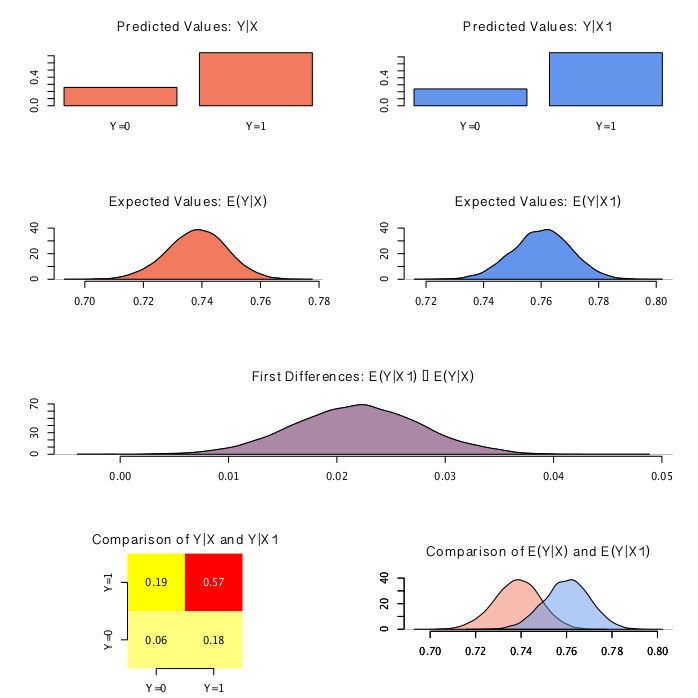
\includegraphics{gr1.png}


\bigskip\hrule{}\bigskip


\emph{Plot of expected values across range of simulations:}

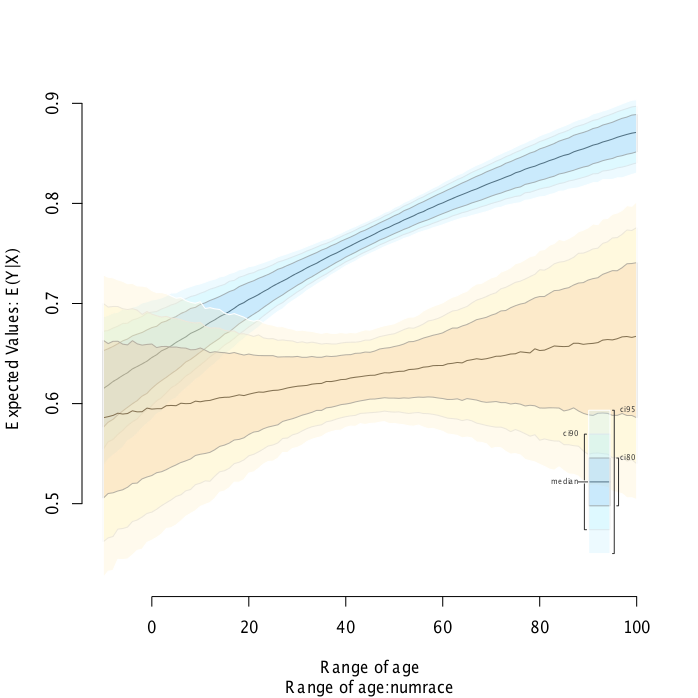
\includegraphics{gr3.png}


\chapter{Frequently Asked Questions}
\label{faq:faq}\label{faq::doc}\label{faq:frequently-asked-questions}
If you find a bug, or cannot figure something out after reading the frequently asked questions below, please send your question to the Zelig listserv at \code{https://groups.google.com/forum/\#!forum/zelig-statistical-software}. Please explain exactly what you did and include the full error message, including the traceback(). You should get an answer from the developers or another user in short order.


\bigskip\hrule{}\bigskip



\section{How do I cite Zelig?}
\label{faq:how-do-i-cite-zelig}
We would appreciate if you would cite Zelig as:
\begin{quote}

Imai, Kosuke, Gary King and Olivia Lau. 2006. “Zelig: Everyone’s Statistical Software,” \href{http://GKing.Harvard.Edu/zelig}{http://GKing.Harvard.Edu/zelig}.
\end{quote}

Please also cite the contributors for the models or methods you are using. These citations can be found in each individual model's vignette which can be found in the the \emph{userguide}.


\bigskip\hrule{}\bigskip



\section{Why can’t I install Zelig?}
\label{faq:why-cant-i-install-zelig}
We recommend that you first check your internet connection, as you must be connected to install packages. In addition, there are a few platform-specific reasons why you may be having installation problems:
\begin{itemize}
\item {} 
\textbf{On Windows}: If you are using the very latest version of R, you may not be able to install Zelig until we update Zelig to work with this latest release. Currently Zelig 5.0.1 is compatible with R(≥ 3.0.2). If you wish to install Zelig in the interim, install the appropriate version of R and try to reinstall Zelig.

\item {} 
\textbf{On Mac or Linux systems}: If you get the following warning message at the end of your installation:

\begin{Verbatim}[commandchars=\\\{\}]
\PYG{o}{\PYGZgt{}} Installation of package VGAM had non\PYG{o}{\PYGZhy{}}zero exit status \PYG{k+kr}{in} \PYG{k+kc}{...}
\end{Verbatim}

this means that you were not able to install VGAM properly. Make sure that you have the g77 Fortran compiler. For Intel Macs, download the Apple developer tools. After installation, try to install Zelig again.

\end{itemize}

If neither solution works, feel free email the Zelig mailing list directly at: \href{https://groups.google.com/forum/\#!forum/zelig-statistical-software}{https://groups.google.com/forum/\#!forum/zelig-statistical-software}.


\bigskip\hrule{}\bigskip



\section{Why can’t I install R?}
\label{faq:why-cant-i-install-r}
If you have problems installing R, you should search the internet for the R help mailing list, check out technical Q \& A forums (e.g., StackOverflow), or email the Zelig mailing list directly at: \href{https://groups.google.com/forum/\#!forum/zelig-statistical-software}{https://groups.google.com/forum/\#!forum/zelig-statistical-software}.


\bigskip\hrule{}\bigskip



\section{Why can’t I load data?}
\label{faq:why-cant-i-load-data}
It is likely that the reason you are unable to load data because you have not specfied the correct working directory (e.g., the location of the data you are trying to load). You should specify you working directory use the \code{setwd()} function in which you will include the the file path to your working director. For example, if I wanted to load a file that is my \emph{Documents} folder, I must first:

\begin{Verbatim}[commandchars=\\\{\}]
\PYG{o}{\PYGZgt{}} setwd\PYG{p}{(}\PYG{l+s}{\PYGZdq{}}\PYG{l+s}{path/to/Documents\PYGZdq{}}\PYG{p}{)}
\end{Verbatim}

File paths can be found by right clicking the workign directory folder in any file browser and clicking ``Get Info'' (on Mac) or ``Properties'' (on Windows). Black-slashes (\textbackslash{}) in file paths copied from the ``Properties'' link on Windows machines must be replace with forward-slashes (/). For example, the Windows path: \code{C:\textbackslash{}Program Files\textbackslash{}R}, would be typed as \code{C:/Program Files/R}.


\bigskip\hrule{}\bigskip



\section{How do I increase the memory for R?}
\label{faq:how-do-i-increase-the-memory-for-r}
Windows users may get the error that R has run out of memory. If you've installed more memory on your machine, you may have to reinstall R in order to take advantage of the additional capacity.

You may also set the amount of available memory manually. Close R, then right-click on your R program icon (the icon on your desktop or in your programs directory). Select “Properties”, and then select the “Shortcut” tab. Look for the “Target” field and after the closing quotes around the location of the R executible, add

\begin{Verbatim}[commandchars=\\\{\}]
\PYG{o}{\PYGZhy{}}\PYG{o}{\PYGZhy{}}max\PYG{o}{\PYGZhy{}}mem\PYG{o}{\PYGZhy{}}size\PYG{o}{=}\PYG{l+m}{500}M
\end{Verbatim}

You may increase this value up to 2GB or the maximum amount of physical RAM you have installed. If you get the error that R cannot allocate a vector of length x, close out of R and add the following line to the “Target” field:

\begin{Verbatim}[commandchars=\\\{\}]
\PYG{o}{\PYGZhy{}}\PYG{o}{\PYGZhy{}}max\PYG{o}{\PYGZhy{}}vsize\PYG{o}{=}\PYG{l+m}{500}M
\end{Verbatim}

or as appropriate.

You can always check to see how much memory R has available by typing at the R prompt

\begin{Verbatim}[commandchars=\\\{\}]
\PYG{o}{\PYGZgt{}} round\PYG{p}{(}memory.limit\PYG{p}{(}\PYG{p}{)}\PYG{o}{/}\PYG{l+m}{2}\PYG{o}{\PYGZca{}}\PYG{l+m}{20}\PYG{p}{,} \PYG{l+m}{2}\PYG{p}{)}
\end{Verbatim}

which gives you the amount of available memory in MB.


\bigskip\hrule{}\bigskip



\section{Why doesn’t the pdf print properly?}
\label{faq:why-doesnt-the-pdf-print-properly}
Zelig uses several special LaTeX environments. If the pdf looks right on the screen, there are two possible reasons why it’s not printing properly:
\begin{itemize}
\item {} 
Adobe Acrobat isn’t cleaning up the document. Updating to Acrobat
Reader 6.0.1 or higher should solve this problem.

\item {} 
Your printer doesn’t support PostScript Type 3 fonts. Updating your
print driver should take care of this problem.

\end{itemize}


\bigskip\hrule{}\bigskip



\section{R is neat. How can I find out more?}
\label{faq:r-is-neat-how-can-i-find-out-more}
R is a collective project with contributors from all over the world. Their website (\href{https://r-project.org}{r-project.org}.) has more information on the R project, R packages, conferences, and other learning material.


\chapter{About Zelig}
\label{about:about}\label{about::doc}\label{about:about-zelig}
Zelig is an open source project development and maintained by the Data Science group at the \href{http://datascience.iq.harvard.edu/}{Data Science group} at Harvard's Institute for Quantative Social Science (IQSS). It was originally concieved and created by Kosuke Imai, Gary King, and Olivia Lau in 2007. The name is borrowed from Woody Allen's movie with the same name, Zelig. Leonard Zelig is a fictional character who takes on the characteristics of any strong personality around. Likewise, the Zelig statistical software easily adapts to any statistical model written in R, and in essence, takes the characteristics of any model.

It leverages (R) code from many researchers and is designed to allow anyone to contribute their methods to it. Hence, we often refer to Zelig as ``everyone's statistical software'' and our aim is to make it, as well as the models it wraps, as accessible as possible. As such, Zelig comes with self-contained documentation that minimizes startup costs, automates model summaries and graphics, and bridges existing R implementations through an intelligble call structure.

\textbf{License:} GPL-2 \textbar{} GPL-3 {[}expanded from: GPL (≥ 2){]}

\textbf{Contact:} For questions, please join the Zelig mailing list:
\href{https://groups.google.com/forum/\#!forum/zelig-statistical-software}{https://groups.google.com/forum/\#!forum/zelig-statistical-software}

\textbf{The Zelig Team:}
\begin{itemize}
\item {} 
Gary King \emph{(Principle Investigator)}

\item {} 
James Honaker \emph{(Project Lead)}

\item {} 
Christine Choirat \emph{(Lead Author)}

\item {} 
Kosku Imai

\item {} 
Olivia Lau

\end{itemize}


\bigskip\hrule{}\bigskip



\section{Technical Vision}
\label{about:technical-vision}
Zelig is a framework for interfacing a wide range of statistical models and analytic methods in a common and simple way. Above and beyond estimation, Zelig adds considerable infrastructure to existing heterogenous R implementations by translating hard-to-interpret coefficients into quanities of interest (e.g., expected and predicted values) through a simple call structure. This includes many specific methods, based on likelihood, frequentist, Bayesian, robust Bayesian and nonparametric theories of inference. Developers are encouraged to add their R packages to the Zelig toolkit by writing a few simple bridge functions.

Additional features include:
\begin{itemize}
\item {} 
Dealing with missing data by combining multiply imputed datasets

\item {} 
Automating statistical bootstrapping

\item {} 
Improving parametric procedures by leveraging nonparametric matching methods

\item {} 
Evaluating counterfactuals

\item {} 
Allowing condtional population and super population inferences

\item {} 
Automating the creation of replication data files

\end{itemize}


\chapter{Model vignettes}
\label{vignette:vignettes}\label{vignette::doc}\label{vignette:model-vignettes}

\bigskip\hrule{}\bigskip



\section{Zelig-ls}
\label{vignette:zelig-ls}
Least Squares Regression for Continuous Dependent Variables

Use least squares regression analysis to estimate the best linear
predictor for the specified dependent variables.


\subsection{Syntax}
\label{vignette:syntax}
\begin{Verbatim}[commandchars=\\\{\}]
z.out \PYG{o}{\PYGZlt{}\PYGZhy{}} zelig\PYG{p}{(}Y \PYG{o}{\PYGZti{}} X1 \PYG{o}{+} X2\PYG{p}{,} model \PYG{o}{=} \PYG{l+s}{\PYGZdq{}}\PYG{l+s}{ls\PYGZdq{}}\PYG{p}{,} data \PYG{o}{=} mydata\PYG{p}{)}
x.out \PYG{o}{\PYGZlt{}\PYGZhy{}} setx\PYG{p}{(}z.out\PYG{p}{)}
s.out \PYG{o}{\PYGZlt{}\PYGZhy{}} sim\PYG{p}{(}z.out\PYG{p}{,} x \PYG{o}{=} x.out\PYG{p}{)}
\end{Verbatim}


\subsection{Examples}
\label{vignette:examples}

\subsubsection{Basic Example with First Differences}
\label{vignette:basic-example-with-first-differences}
Attach sample data:

\begin{Verbatim}[commandchars=\\\{\}]
library\PYG{p}{(}Zelig5\PYG{p}{)}
\end{Verbatim}

\begin{Verbatim}[commandchars=\\\{\}]
\PYG{c}{\PYGZsh{}\PYGZsh{} Loading required package: methods}
\PYG{c}{\PYGZsh{}\PYGZsh{} Loading required package: MASS}
\PYG{c}{\PYGZsh{}\PYGZsh{} Loading required package: survival}
\PYG{c}{\PYGZsh{}\PYGZsh{} Loading required package: splines}
\PYG{c}{\PYGZsh{}\PYGZsh{} Loading required package: VGAM}
\PYG{c}{\PYGZsh{}\PYGZsh{} Loading required package: stats4}
\PYG{c}{\PYGZsh{}\PYGZsh{} Loading required package: jsonlite}
\PYG{c}{\PYGZsh{}\PYGZsh{}}
\PYG{c}{\PYGZsh{}\PYGZsh{} Attaching package: \PYGZsq{}jsonlite\PYGZsq{}}
\PYG{c}{\PYGZsh{}\PYGZsh{}}
\PYG{c}{\PYGZsh{}\PYGZsh{} The following object is masked from \PYGZsq{}package:utils\PYGZsq{}:}
\PYG{c}{\PYGZsh{}\PYGZsh{}}
\PYG{c}{\PYGZsh{}\PYGZsh{}     View}
\PYG{c}{\PYGZsh{}\PYGZsh{}}
\PYG{c}{\PYGZsh{}\PYGZsh{} Loading required package: AER}
\PYG{c}{\PYGZsh{}\PYGZsh{} Loading required package: car}
\PYG{c}{\PYGZsh{}\PYGZsh{}}
\PYG{c}{\PYGZsh{}\PYGZsh{} Attaching package: \PYGZsq{}car\PYGZsq{}}
\PYG{c}{\PYGZsh{}\PYGZsh{}}
\PYG{c}{\PYGZsh{}\PYGZsh{} The following object is masked from \PYGZsq{}package:VGAM\PYGZsq{}:}
\PYG{c}{\PYGZsh{}\PYGZsh{}}
\PYG{c}{\PYGZsh{}\PYGZsh{}     logit}
\PYG{c}{\PYGZsh{}\PYGZsh{}}
\PYG{c}{\PYGZsh{}\PYGZsh{} Loading required package: lmtest}
\PYG{c}{\PYGZsh{}\PYGZsh{} Loading required package: zoo}
\PYG{c}{\PYGZsh{}\PYGZsh{}}
\PYG{c}{\PYGZsh{}\PYGZsh{} Attaching package: \PYGZsq{}zoo\PYGZsq{}}
\PYG{c}{\PYGZsh{}\PYGZsh{}}
\PYG{c}{\PYGZsh{}\PYGZsh{} The following objects are masked from \PYGZsq{}package:base\PYGZsq{}:}
\PYG{c}{\PYGZsh{}\PYGZsh{}}
\PYG{c}{\PYGZsh{}\PYGZsh{}     as.Date, as.Date.numeric}
\PYG{c}{\PYGZsh{}\PYGZsh{}}
\PYG{c}{\PYGZsh{}\PYGZsh{}}
\PYG{c}{\PYGZsh{}\PYGZsh{} Attaching package: \PYGZsq{}lmtest\PYGZsq{}}
\PYG{c}{\PYGZsh{}\PYGZsh{}}
\PYG{c}{\PYGZsh{}\PYGZsh{} The following object is masked from \PYGZsq{}package:VGAM\PYGZsq{}:}
\PYG{c}{\PYGZsh{}\PYGZsh{}}
\PYG{c}{\PYGZsh{}\PYGZsh{}     lrtest}
\PYG{c}{\PYGZsh{}\PYGZsh{}}
\PYG{c}{\PYGZsh{}\PYGZsh{} Loading required package: sandwich}
\PYG{c}{\PYGZsh{}\PYGZsh{}}
\PYG{c}{\PYGZsh{}\PYGZsh{} Attaching package: \PYGZsq{}AER\PYGZsq{}}
\PYG{c}{\PYGZsh{}\PYGZsh{}}
\PYG{c}{\PYGZsh{}\PYGZsh{} The following object is masked from \PYGZsq{}package:VGAM\PYGZsq{}:}
\PYG{c}{\PYGZsh{}\PYGZsh{}}
\PYG{c}{\PYGZsh{}\PYGZsh{}     tobit}
\PYG{c}{\PYGZsh{}\PYGZsh{}}
\PYG{c}{\PYGZsh{}\PYGZsh{} Loading required package: plyr}
\PYG{c}{\PYGZsh{}\PYGZsh{} Loading required package: dplyr}
\PYG{c}{\PYGZsh{}\PYGZsh{}}
\PYG{c}{\PYGZsh{}\PYGZsh{} Attaching package: \PYGZsq{}dplyr\PYGZsq{}}
\PYG{c}{\PYGZsh{}\PYGZsh{}}
\PYG{c}{\PYGZsh{}\PYGZsh{} The following objects are masked from \PYGZsq{}package:plyr\PYGZsq{}:}
\PYG{c}{\PYGZsh{}\PYGZsh{}}
\PYG{c}{\PYGZsh{}\PYGZsh{}     arrange, desc, failwith, id, mutate, summarise, summarize}
\PYG{c}{\PYGZsh{}\PYGZsh{}}
\PYG{c}{\PYGZsh{}\PYGZsh{} The following object is masked from \PYGZsq{}package:MASS\PYGZsq{}:}
\PYG{c}{\PYGZsh{}\PYGZsh{}}
\PYG{c}{\PYGZsh{}\PYGZsh{}     select}
\PYG{c}{\PYGZsh{}\PYGZsh{}}
\PYG{c}{\PYGZsh{}\PYGZsh{} The following objects are masked from \PYGZsq{}package:stats\PYGZsq{}:}
\PYG{c}{\PYGZsh{}\PYGZsh{}}
\PYG{c}{\PYGZsh{}\PYGZsh{}     filter, lag}
\PYG{c}{\PYGZsh{}\PYGZsh{}}
\PYG{c}{\PYGZsh{}\PYGZsh{} The following objects are masked from \PYGZsq{}package:base\PYGZsq{}:}
\PYG{c}{\PYGZsh{}\PYGZsh{}}
\PYG{c}{\PYGZsh{}\PYGZsh{}     intersect, setdiff, setequal, union}
\end{Verbatim}

\begin{Verbatim}[commandchars=\\\{\}]
\PYG{c}{\PYGZsh{}\PYGZsh{} Warning: replacing previous import by \PYGZsq{}VGAM::show\PYGZsq{} when loading \PYGZsq{}Zelig5\PYGZsq{}}
\PYG{c}{\PYGZsh{}\PYGZsh{} Warning: replacing previous import by \PYGZsq{}AER::tobit\PYGZsq{} when loading \PYGZsq{}Zelig5\PYGZsq{}}
\PYG{c}{\PYGZsh{}\PYGZsh{} Warning: replacing previous import by \PYGZsq{}quantreg::untangle.specials\PYGZsq{} when loading \PYGZsq{}Zelig5\PYGZsq{}}
\PYG{c}{\PYGZsh{}\PYGZsh{} Warning: replacing previous import by \PYGZsq{}dplyr::arrange\PYGZsq{} when loading \PYGZsq{}Zelig5\PYGZsq{}}
\PYG{c}{\PYGZsh{}\PYGZsh{} Warning: replacing previous import by \PYGZsq{}dplyr::desc\PYGZsq{} when loading \PYGZsq{}Zelig5\PYGZsq{}}
\PYG{c}{\PYGZsh{}\PYGZsh{} Warning: replacing previous import by \PYGZsq{}dplyr::failwith\PYGZsq{} when loading \PYGZsq{}Zelig5\PYGZsq{}}
\PYG{c}{\PYGZsh{}\PYGZsh{} Warning: replacing previous import by \PYGZsq{}dplyr::id\PYGZsq{} when loading \PYGZsq{}Zelig5\PYGZsq{}}
\PYG{c}{\PYGZsh{}\PYGZsh{} Warning: replacing previous import by \PYGZsq{}dplyr::mutate\PYGZsq{} when loading \PYGZsq{}Zelig5\PYGZsq{}}
\PYG{c}{\PYGZsh{}\PYGZsh{} Warning: replacing previous import by \PYGZsq{}dplyr::select\PYGZsq{} when loading \PYGZsq{}Zelig5\PYGZsq{}}
\PYG{c}{\PYGZsh{}\PYGZsh{} Warning: replacing previous import by \PYGZsq{}dplyr::summarise\PYGZsq{} when loading \PYGZsq{}Zelig5\PYGZsq{}}
\PYG{c}{\PYGZsh{}\PYGZsh{} Warning: replacing previous import by \PYGZsq{}dplyr::summarize\PYGZsq{} when loading \PYGZsq{}Zelig5\PYGZsq{}}
\PYG{c}{\PYGZsh{}\PYGZsh{} Warning: replacing previous import by \PYGZsq{}methods::setRefClass\PYGZsq{} when loading \PYGZsq{}Zelig5\PYGZsq{}}
\end{Verbatim}

\begin{Verbatim}[commandchars=\\\{\}]
data\PYG{p}{(}macro\PYG{p}{)}
\end{Verbatim}

Estimate model:

\begin{Verbatim}[commandchars=\\\{\}]
z.out1 \PYG{o}{\PYGZlt{}\PYGZhy{}} zelig\PYG{p}{(}unem \PYG{o}{\PYGZti{}} gdp \PYG{o}{+} capmob \PYG{o}{+} trade\PYG{p}{,} model \PYG{o}{=} \PYG{l+s}{\PYGZdq{}}\PYG{l+s}{ls\PYGZdq{}}\PYG{p}{,} data \PYG{o}{=} macro\PYG{p}{)}
\end{Verbatim}

\begin{Verbatim}[commandchars=\\\{\}]
\PYG{c}{\PYGZsh{}\PYGZsh{} How to cite this model in Zelig:}
\PYG{c}{\PYGZsh{}\PYGZsh{}   Kosuke Imai, Gary King, and Olivia Lau. 2007.}
\PYG{c}{\PYGZsh{}\PYGZsh{}   ls: Least Squares Regression for Continuous Dependent Variables}
\PYG{c}{\PYGZsh{}\PYGZsh{}   in Kosuke Imai, Gary King, and Olivia Lau, \PYGZdq{}Zelig: Everyone\PYGZsq{}s Statistical Software,\PYGZdq{}}
\PYG{c}{\PYGZsh{}\PYGZsh{}   http://datascience.iq.harvard.edu/zelig}
\end{Verbatim}

Summarize regression coefficients:

\begin{Verbatim}[commandchars=\\\{\}]
summary\PYG{p}{(}z.out1\PYG{p}{)}
\end{Verbatim}

\begin{Verbatim}[commandchars=\\\{\}]
\PYG{c}{\PYGZsh{}\PYGZsh{} Model: 1}
\PYG{c}{\PYGZsh{}\PYGZsh{} Call:}
\PYG{c}{\PYGZsh{}\PYGZsh{} stats::lm(formula = unem \PYGZti{} gdp + capmob + trade, data = .)}
\PYG{c}{\PYGZsh{}\PYGZsh{}}
\PYG{c}{\PYGZsh{}\PYGZsh{} Coefficients:}
\PYG{c}{\PYGZsh{}\PYGZsh{} (Intercept)          gdp       capmob        trade}
\PYG{c}{\PYGZsh{}\PYGZsh{}      6.1813      \PYGZhy{}0.3236       1.4219       0.0199}
\PYG{c}{\PYGZsh{}\PYGZsh{}}
\PYG{c}{\PYGZsh{}\PYGZsh{} Next step: Use \PYGZsq{}setx\PYGZsq{} method}
\end{Verbatim}

Set explanatory variables to their default (mean/mode) values, with high (80th percentile) and low (20th percentile) values for the trade variable:

\begin{Verbatim}[commandchars=\\\{\}]
x.high \PYG{o}{\PYGZlt{}\PYGZhy{}} setx\PYG{p}{(}z.out1\PYG{p}{,} trade \PYG{o}{=} quantile\PYG{p}{(}macro\PYG{o}{\PYGZdl{}}trade\PYG{p}{,} \PYG{l+m}{0.8}\PYG{p}{)}\PYG{p}{)}
x.low \PYG{o}{\PYGZlt{}\PYGZhy{}} setx\PYG{p}{(}z.out1\PYG{p}{,} trade \PYG{o}{=} quantile\PYG{p}{(}macro\PYG{o}{\PYGZdl{}}trade\PYG{p}{,} \PYG{l+m}{0.2}\PYG{p}{)}\PYG{p}{)}
\end{Verbatim}

Generate first differences for the effect of high versus low trade on GDP:

\begin{Verbatim}[commandchars=\\\{\}]
s.out1 \PYG{o}{\PYGZlt{}\PYGZhy{}} sim\PYG{p}{(}z.out1\PYG{p}{,} x \PYG{o}{=} x.high\PYG{p}{,} x1 \PYG{o}{=} x.low\PYG{p}{)}
\end{Verbatim}


\subsubsection{Using Dummy Variables}
\label{vignette:using-dummy-variables}
Estimate a model with fixed effects for each country (see for help
with dummy variables). Note that you do not need to create dummy
variables, as the program will automatically parse the unique values
in the selected variable into discrete levels.

\begin{Verbatim}[commandchars=\\\{\}]
z.out2 \PYG{o}{\PYGZlt{}\PYGZhy{}} zelig\PYG{p}{(}unem \PYG{o}{\PYGZti{}} gdp \PYG{o}{+} trade \PYG{o}{+} capmob \PYG{o}{+} country\PYG{p}{,}
                model \PYG{o}{=} \PYG{l+s}{\PYGZdq{}}\PYG{l+s}{ls\PYGZdq{}}\PYG{p}{,} data \PYG{o}{=} macro\PYG{p}{)}
\end{Verbatim}

\begin{Verbatim}[commandchars=\\\{\}]
\PYG{c}{\PYGZsh{}\PYGZsh{} How to cite this model in Zelig:}
\PYG{c}{\PYGZsh{}\PYGZsh{}   Kosuke Imai, Gary King, and Olivia Lau. 2007.}
\PYG{c}{\PYGZsh{}\PYGZsh{}   ls: Least Squares Regression for Continuous Dependent Variables}
\PYG{c}{\PYGZsh{}\PYGZsh{}   in Kosuke Imai, Gary King, and Olivia Lau, \PYGZdq{}Zelig: Everyone\PYGZsq{}s Statistical Software,\PYGZdq{}}
\PYG{c}{\PYGZsh{}\PYGZsh{}   http://datascience.iq.harvard.edu/zelig}
\end{Verbatim}

\begin{Verbatim}[commandchars=\\\{\}]
z.out3 \PYG{o}{\PYGZlt{}\PYGZhy{}} zelig\PYG{p}{(}unem \PYG{o}{\PYGZti{}} gdp \PYG{o}{+} trade \PYG{o}{+} capmob \PYG{o}{+} as.factor\PYG{p}{(}country\PYG{p}{)}\PYG{p}{,}
                model \PYG{o}{=} \PYG{l+s}{\PYGZdq{}}\PYG{l+s}{ls\PYGZdq{}}\PYG{p}{,} data \PYG{o}{=} macro\PYG{p}{)}
\end{Verbatim}

\begin{Verbatim}[commandchars=\\\{\}]
\PYG{c}{\PYGZsh{}\PYGZsh{} How to cite this model in Zelig:}
\PYG{c}{\PYGZsh{}\PYGZsh{}   Kosuke Imai, Gary King, and Olivia Lau. 2007.}
\PYG{c}{\PYGZsh{}\PYGZsh{}   ls: Least Squares Regression for Continuous Dependent Variables}
\PYG{c}{\PYGZsh{}\PYGZsh{}   in Kosuke Imai, Gary King, and Olivia Lau, \PYGZdq{}Zelig: Everyone\PYGZsq{}s Statistical Software,\PYGZdq{}}
\PYG{c}{\PYGZsh{}\PYGZsh{}   http://datascience.iq.harvard.edu/zelig}
\end{Verbatim}

\begin{Verbatim}[commandchars=\\\{\}]
x.US \PYG{o}{\PYGZlt{}\PYGZhy{}} setx\PYG{p}{(}z.out3\PYG{p}{,} country \PYG{o}{=} \PYG{l+s}{\PYGZdq{}}\PYG{l+s}{United States\PYGZdq{}}\PYG{p}{)}
\end{Verbatim}

Set values for the explanatory variables, using the default
mean/mode values, with country set to the United States and Japan,
respectively:

\begin{Verbatim}[commandchars=\\\{\}]
x.US \PYG{o}{\PYGZlt{}\PYGZhy{}} setx\PYG{p}{(}z.out2\PYG{p}{,} country \PYG{o}{=} \PYG{l+s}{\PYGZdq{}}\PYG{l+s}{United States\PYGZdq{}}\PYG{p}{)}
x.Japan \PYG{o}{\PYGZlt{}\PYGZhy{}} setx\PYG{p}{(}z.out2\PYG{p}{,} country \PYG{o}{=} \PYG{l+s}{\PYGZdq{}}\PYG{l+s}{Japan\PYGZdq{}}\PYG{p}{)}
\end{Verbatim}

Simulate quantities of interest:

\begin{Verbatim}[commandchars=\\\{\}]
s.out2 \PYG{o}{\PYGZlt{}\PYGZhy{}} sim\PYG{p}{(}z.out2\PYG{p}{,} x.US\PYG{p}{,} x.Japan\PYG{p}{)}
\end{Verbatim}

\begin{Verbatim}[commandchars=\\\{\}]
plot\PYG{p}{(}s.out2\PYG{p}{)}
\end{Verbatim}
\begin{figure}[htbp]
\centering
\capstart

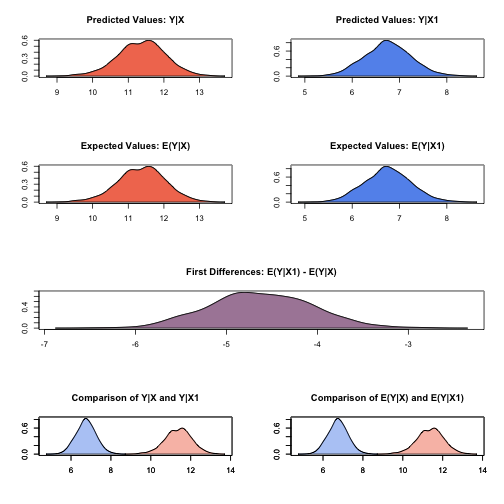
\includegraphics{unnamed-chunk-12.png}
\caption{plot of chunk unnamed-chunk-12}\end{figure}


\subsection{Model}
\label{vignette:model}\begin{itemize}
\item {} 
The \emph{stochastic component} is described by a density with mean
\$mu\_i\$ and the common variance \$sigma\textasciicircum{}2\$

\$\$Y\_i ; sim ; f(y\_i mid mu\_i, sigma\textasciicircum{}2).\$\$

\item {} 
The \emph{systematic component} models the conditional mean as

\$\$mu\_i =  x\_i beta\$\$

where \$x\_i\$ is the vector of covariates, and \$beta\$ is the vector
of coefficients.

The least squares estimator is the best linear predictor of a
dependent variable given \$x\_i\$, and minimizes the sum of squared
residuals, \$sum\_\{i=1\}\textasciicircum{}n (Y\_i-x\_i beta)\textasciicircum{}2\$.

\end{itemize}


\subsection{Quantities of Interest}
\label{vignette:quantities-of-interest}\begin{itemize}
\item {} 
The expected value (\emph{qi\$ev}) is the mean of simulations
from the stochastic component,

\$\$E(Y) = x\_i beta,\$\$

given a draw of \$beta\$ from its sampling distribution.

\item {} 
In conditional prediction models, the average expected treatment
effect (\emph{att.ev}) for the treatment group is
\begin{description}
\item[{\$\$frac\{1\}\{sum\_\{i=1\}\textasciicircum{}n t\_i\}sum\_\{i:t\_i=1\}\textasciicircum{}n left\{ Y\_i(t\_i=1) -}] \leavevmode
E{[}Y\_i(t\_i=0){]} right\},\$\$

\end{description}

where \$t\_i\$ is a binary explanatory variable defining the treatment
(\$t\_i=1\$) and control (\$t\_i=0\$) groups. Variation in the simulations
are due to uncertainty in simulating \$E{[}Y\_i(t\_i=0){]}\$, the
counterfactual expected value of \$Y\_i\$ for observations in the
treatment group, under the assumption that everything stays the same
except that the treatment indicator is switched to \$t\_i=0\$.

\end{itemize}


\subsection{Output Values}
\label{vignette:output-values}
The output of each Zelig command contains useful information which you
may view. For example, if you run
\emph{z.out \textless{}- zelig(y \textasciitilde{} x, model = ls, data)}, then you may examine the
available information in \emph{z.out} by using \emph{names(z.out)}, see the
\emph{coefficients} by using \emph{z.out\$coefficients}, and
a default summary of information through \emph{summary(z.out)}. Other
elements available through the \emph{\$} operator are listed
below.


\subsection{See also}
\label{vignette:see-also}
The least squares regression is part of the stats package by William N.
Venables and Brian D. Ripley {[}@VenRip02{]}. In addition, advanced users may
wish to refer to \emph{help(lm)} and \emph{help(lm.fit)}. Robust standard errors
are implemented via the sandwich package by Achim Zeileis
{[}@Zeileis04{]}. Sample data are from @KinTomWit00.



\renewcommand{\indexname}{Index}
\printindex
\end{document}
